\chapter{Fejlesztői dokumentáció}
\label{ch:impl}

\section{A feladat specifikálása}
A beépülő modul célja a téradatok verziókezelésének megvalósítása a \emph{QGIS}-en belül az \emph{AEGIS} keretrendszer segítségével. Ez szétválasztható egy \emph{back-end} részre, ami a verziókezelésért valamint az adatok és transzformációk tárolásáért felel, és egy \emph{front-end} részre, ami egyrészt grafikus felhasználói felületet biztosít, valamint felel az adatreprezentációs és architekturális különbségek áthidalásáért.

\begin{figure}[H]
	\centering
	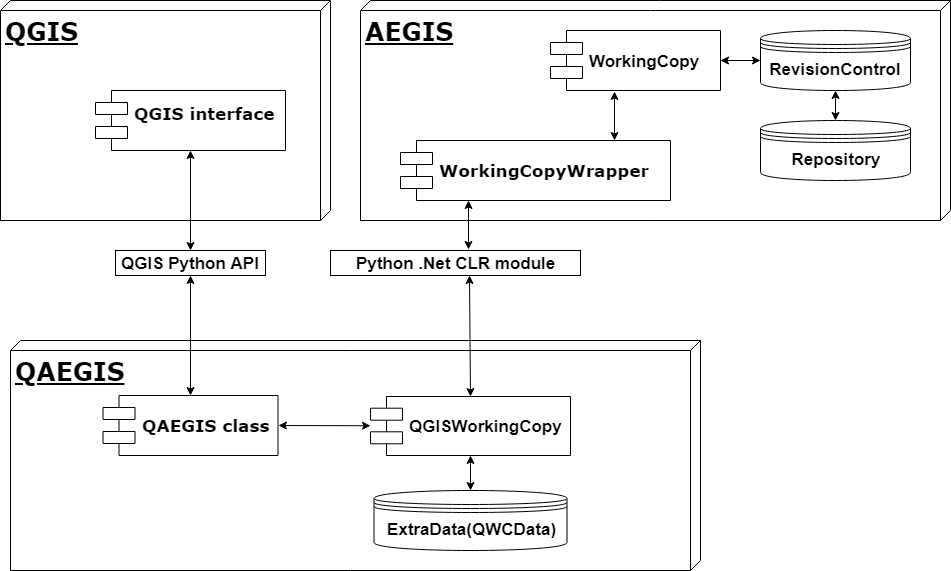
\includegraphics[width=0.8\textwidth,height=220px]{images/qaegis_component_diagram.png}
	\caption{A program komponensdiagramja}
	\label{fig:picture-7}
\end{figure}

\subsection{A geometriaadatok kezelése}
A geometriák tárolása, betöltése, valamint eltávolításuk kezelése mind az \emph{AEGIS} létező funkciói voltak a projekt kezdeténél, így a tényleges feladat, a transzformációk definiálása, és létrehozása.
Az átalakítások tervezése közben az a fő szempont, hogy a lehető legáltalánosabbak legyenek, és minden lehetséges módosítás leírható legyen véges alkalmazásukkal. Ezt a törekvést segíti az, hogy az \emph{AEGIS} geometriatípusai megfelelnek a \emph{Simple Feature Access} (röviden \emph{SFA}) standardnak \cite{sfa}. Az \emph{SFA} modell rendelkezik egy geometria ősosztállyal, így egy teljes leszármazási hierarchia adott, minden geometriának van közös ős típusa. Ezáltal a geometriák a következő hierarchiával rendelkeznek: a pontok különálló típust képeznek, a vonalláncok koordináták sorozatai, amik hasonlóan viselkednek a pontokhoz, a sokszögek pedig gyűrűkkel vannak leírva, amik a vonalak speciális változatai, így az "alacsonyabb szintű" geometriák transzformációi felhasználhatóak a bonyolultabb térobjektumok átalakításainak leírásához is. 
\begin{note}
A \emph{Simple Feature Access} geometriák tárolására és elérésére kialakított két részből álló szabvány. Az első rész (\emph{SFA-CA} azaz \emph{Common Architecture}) egy modellt definiál a két dimenziós geometriáknak pontok közti lineáris interpolációval. Ez a rész definiálja WKT és WKB szabványos reprezentációkat is. A második rész a szabvány SQL alapú implementációját írja le. Az SFA standard az OGC (\emph{Open Geospatial Consortium}) és az ISO (\emph{International Organization for Standardization}) szervezetek által elfogadott.
\begin{figure}[H]
	\centering
	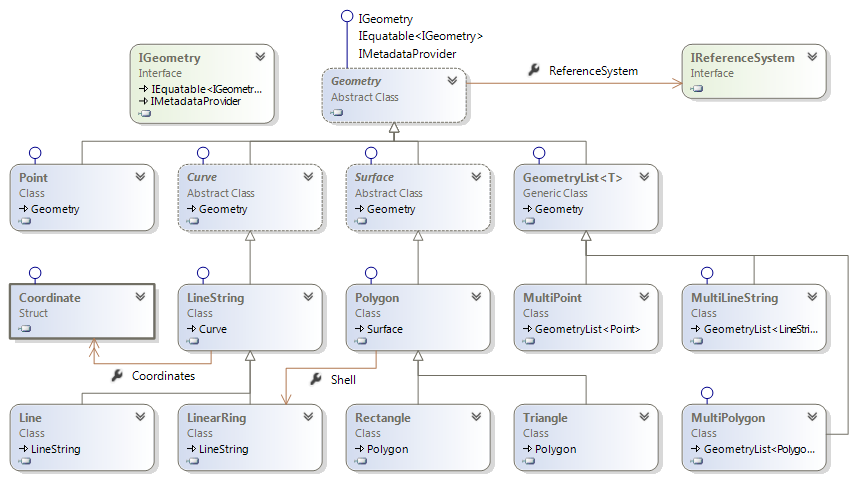
\includegraphics[width=0.8\textwidth,height=220px]{images/sfa.png}
	\caption{A \emph{Simple Feature Access} objektum-relációs modellje az AEGIS-ben}
	\label{fig:picture-8}
\end{figure}
\end{note}

 Az alakzatok lehetséges változásainak megfelelő rekreálásához a következő transzformációkat szükséges definiálni:
\begin{itemize}
	\item Pont eltolása
	\item Vonal részleges vagy teljes eltolása
	\item Pont felvétele a vonalba
	\item Pont eltávolítása a vonalból
	\item Sokszög héjának módosítása
	\item Sokszögben lévő lyuk módosítása
	\item Lyuk felvétele sokszögbe
	\item Lyuk eltávolítása sokszögből
\end{itemize}
Ezeken kívül az összes többi alakzatot egybefogó, úgynevezett multigeometriák változásainak leírásához szükségesek a következő műveletek:
\begin{itemize}
	\item Multigeometria egy vagy több részének módosítása a megfelelő egyedi geometria transzformációkkal
	\item Geometria hozzáadása multigeometriához
	\item Geometria eltávolítása multigeometriából
\end{itemize}
Ezen transzformációk segítségével bármilyen alapvető geometriaváltozást le lehet írni.

A transzformációk generálása komplex feladat, melynek során elemeznünk kell a kiindulási geometriát, és a végeredményt, ez alapján pedig létrehozni azt a transzformációgyűjteményt amit végrehajtva az eredetin, megkapjuk az újat. Vonalláncokra és poligonokra a következő algoritmussal adható meg:
\begin{enumerate}
	\item Tekintsük az eredeti és a módosult geometria komponenseinek számát (ld. \ref{sec:definitions}.~szakasz)
	\item A két geometria megegyező hosszú részein -- ami megegyezik a komponensszámuk minimumával -- hozzuk létre azokat a transzformációkat, amik az eredeti részeit az új részeknek megfelelő részekre alakítják
	\item Amennyiben az új geometria hosszabb, a régiben még nem létező részeket adjuk hozzá
	\item Amennyiben a régi geometria hosszabb, az újban már nem létező részeket töröljük ki
\end{enumerate}

Mivel pont geometriáknál csak az eltolás művelete létezik, nem szükséges részekre bontani a transzformációgenerálást, a koordináták különbségeiből kiszámolható az összes szükséges paraméter.

Ezen részek implementálásával a geometriák alakulásának követése megvalósítható.

\subsection{A \emph{QGIS} reprezentáció kezelése}
A fő különbség az \emph{AEGIS} és a \emph{QGIS} geometriákat kezelő része között az, hogy az előbbi csak a téradatot kezeli, az utóbbi viszont ezeket még rétegekre osztva jeleníti meg. Ezzel önmagában nem lenne probléma, viszont a \emph{QGIS} nem rendel egyedi azonosítót a geometriákhoz, így előfordulhat, hogy két különböző rétegen azonos geometria szerepel, és módosításukkor nem tudjuk megállapítani, hogy az \emph{AEGIS}-ben tárolt adatok közül melyik módosult. Ez alapján  a beépülő modulon belül megvalósítandó plusz funkciók a következőek:
\begin{itemize}
	\item A \emph{QGIS} objektumok (feature-ök) és az \emph{AEGIS} geometriák kapcsolatának nyilvántartása
	\item A \emph{QGIS} műveleteinek megfeleltetése az \emph{AEGIS} műveleteknek
	\item Az \emph{AEGIS}-ben tárolt állapotok megjelenítése 
	\item A verziókezelés lépéseihez grafikus kezelőfelület biztosítása
\end{itemize}

\section{Geometriai adatok változásának kezelése}
\subsection{Az \emph{AEGIS} WorkingCopy}
Az \emph{AEGIS} verziókezelő moduljának külső interfésze az úgynevezett \texttt{Working Copy}, avagy munkapéldány. Ezen kereszült a következő funkciók érhetőek el:
\begin{enumerate}
	\item Teljes revíziókezelő, és hozzá tartozó tároló létrehozása vagy betöltése, attól függően, hogy van-e már jelen egy
	\item Geometriák hozzáadása az aktuális verzióhoz
	\item Geometriák eltávolítása az aktuális verzióból
	\item Geometria módosítása az aktuális verzióban, az \texttt{IGeometryTransformation} interfészt megvalósító transzformációpéldánnyal
	\item Aktuális verzió mentése a verziókezelőbe
	\item Tetszőleges verzió betöltése és megjelenítése
\end{enumerate}
A \texttt{WorkingCopy} két hiányossággal rendelkezik a beépülő modulban való használathoz. Transzformációk előállítását nem támogatja, valamint az aktuális állapotát kifelé csak geometriák halmazaként biztosítja, ami a \emph{QGIS} réteges megjelenítésében problémákat okozhat.
\subsection{Az AEGIS WorkingCopyWrapper}
A munkapéldány említett hiányosságainak pótlására jött létre a \texttt{WorkingCopyWrapper} osztály, amely a \texttt{WorkingCopy}-hoz képest az alábbi többletfunkciókkal bír:
\begin{enumerate}
	\item Eredeti és módosult geometria alapján transzformációk generálása, majd ezzel a \emph{WorkingCopy} módosító függvényének használata
	\item Egy egyedi azonosítókkal ellátott geometrialista biztosítása a lokális állapotról
\end{enumerate}
A szükséges transzformációkat és generálásukat az \emph{AEGIS Processing} könyvtárában kellett implementálni.
\subsection{A transzformációk}
A geometriák átalakító műveletek kialakítása az alábbi elven alapul:
\begin{itemize}
	\item A pontok transzformációja leírható egy egyszerű vektor hozzáadással
	\item Az összes többi geometria kisebb részekből áll (ld. \ref{sec:definitions}.~szakasz)
	\item Egy geometria módosítása leírható a részeire vonatkozó kisebb transzformációkkal
\end{itemize}
Ez alapján három típusú transzformáció alakult ki: $i)$ a rész módosítása, ami a módosítandó részek indexeit és a részeken elvégzendő résztranszformációit tartalmazza; $ii)$ a rész hozzáadása amely az új rész geometriáját és a beszúrás indexét tartalmazza; $iii)$ valamint a rész eltávolítása, amely az eltávolítandó rész indexét tárolja, valamint az eltávolított rész geometriáját, erre az invertálhatóság megvalósításához van szükség.
\subsection{Az \texttt{IGeometryTransformation} interfész}
Ahogy korábban is említésre került, az \emph{AEGIS} a transzformációkat az \texttt{IGeometryTransformation} implementációjaként várja. 
\begin{figure}[H]
	\centering
	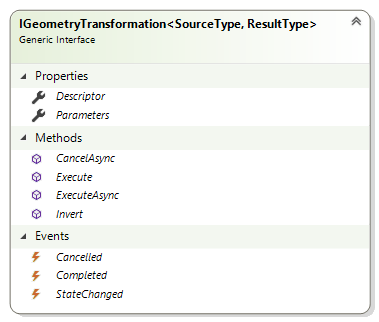
\includegraphics[width=0.85\textwidth,height=240px]{images/GeomTransformIface.png}
	\caption{A geometriatranszformációs interfész osztálydiagramja}
	\label{fig:picture-9}
\end{figure}
Ezen interfész legfontosabb metódusai:
\begin{enumerate}
	\item \texttt{Execute(IGeometry geometry)}: a transzformáció végrehajtása az \texttt{IGeometry} interfésznek megfelelő téradaton, a módosított alakzat visszaadása. A forrásgeometriának meg kell egyeznie a transzformáció bemeneti típusával.
	\item \texttt{Invert()}: A transzformáció inverzének előállítása, mellyel helyreállítható az eredeti geometria. Hozzáadás típusú művelet inverze ugyanazon az indexen történő eltávolítás és fordítva, részmódosítás esetén a résztranszformációk inverzeinek végrehajtása ugyanazokon a részeken.
\end{enumerate}
Az összes módosítást leíró osztály rendelkezik ezen metódusok egyedi implementációival, melyek megfelelnek a saját geometriatípusaiknak.
\subsection{A transzformációk generálása}
Az eredeti és módosított geometriákból transzformációk generálását az \emph{AEGIS Processing} modulban található \texttt{TransformationFactory} statikus osztályok végzik.
A transzformációk létrehozása a specifikációban leírt algoritmus alapján működik, ez az alábbi pseudokóddal szemléltethető:
\begingroup
\begin{algorithm}[H]
	\caption{The general transformation list generating algorithm} 
	\label{alg:transformgen} 
	\textbf{\underline{Funct}} CreateTransformation($old\_geometry,new\_geometry$)
	\begin{algorithmic}[1] % sorszámok megjelenítése minden n. sor előtt, most n = 1
		\STATE Set number of parts in old geometry ${\cal C}_{old}$ := \texttt{old\_geometry.Count} and the number of parts in new geometry ${\cal C}_{new}$ :=  \texttt{new\_geometry.Count}
		\STATE Set result transformation list ${\cal L}_{result}$ := $\{\}$
		\FOR{$i=0,\ldots,\min({\cal C}_{old},{\cal C}_{new})$}
			\STATE Generate \texttt{partial\_transformation} from \texttt{old\_geometry[i]} and \texttt{new\_geometry[i]}
			\STATE Store \texttt{partial\_transformation} in ${\cal L}_{result}$
		\ENDFOR
		\FOR{$i={\cal C}_{old},\ldots,{\cal C}_{new}$}
			\STATE Generate \texttt{part\_addition\_transformation} from \texttt{new\_geometry[i]}
			\STATE Store \texttt{part\_addition\_transformation} in ${\cal L}_{result}$
		\ENDFOR
		\FOR{$i={\cal C}_{new},\ldots,{\cal C}_{old}$}
		\STATE Generate \texttt{part\_removal\_transformation} from \texttt{old\_geometry[i]}
		\STATE Store \texttt{part\_removal\_transformation} in ${\cal L}_{result}$
		\ENDFOR
		\STATE \textbf{return} ${\cal L}_{result}$
	\end{algorithmic}
\end{algorithm}

\endgroup
Mint látható, a generáló függvény először létrehoz annyi résztranszformációt, amekkora részen még egyezik a két geometria hossza, majd a még nem, vagy már nem jelen lévő részgeometriák létrehozásának illetve eltávolításának műveleteit állítja elő. Az összes transzformációgenerátor hasonló módon működik.

\section{C\# folyamatok használata Python kódban}
Ahogy a specifikáció elején említésre került, a szoftver amihez a verziókezelő beépülő modul és a verziókezelést biztosító könyvtár két teljesen különböző technológiát használ. Mivel a Python programozási nyelv széleskörűen elterjedt különböző extra funkciók hozzáadására más környezetekhez, ezért több opció volt az eltérő megoldások összekötésére. Az egyik az \emph{IronPython} nevű kiegészítő modul a Pythonhoz, viszon ez csak a nyelv 2.7-es verzióját támogatja, aminek hamarosan megszűnik a támogatottsága, így más utat kellett keresni. Az előbbihez hasonlóan nyílt forráskódú \emph{Python.NET} modul azonos funkcionalitással rendelkezik, és a legújabb verziókkal is kompatibilis, így kézenfekvő megoldásnak bizonyult. A \emph{Python.NET} projekt integrálása a \emph{QGIS} pluginba egyedül azért okozott nehézséget, mivel a nyelvi összeköttetést biztosító szoftver fordításához számos dependenciának jelen kell lennie a rendszerben, így végül már fordított bináris formájában került a beépülő modulba. Ez sajnos kizárja annak lehetőségét, hogy a könyvtár esetleges frissülésével a plugin is dinamikusan megkapja a legújabb állományokat, viszont a program telepítését meglehetősen megkönnyíti.
\subsection{A \emph{Python.NET} használata}
A \emph{Python.NET} az úgynevezett \emph{Common Language Runtime} (\emph{CLR}) modult biztosítja a Python programozási nyelvhez. Amennyiben a fordított források a Python belső elérési útvonalain szerepelnek, importálható a CLR modul. Ezután a szintén classpathhoz adott dinamikusan linkelhető szoftverkönyvtárba (DLL) fordított C\# könyvtárakat is hozzáadhatjuk a Python kódhoz. A tényleges implementációban a beágyazás az alábbi módon néz ki :
\lstset{caption={A CLR modul bekötése, és a DLL fájlok importálása a Q-Aegis kódjában}, label=src:pythonload}
\begin{lstlisting}[language={python}]
pluginpath = "{}/../python/plugins/qaegis".format(QgsApplication.pluginPath())
sys.path.insert(0,pluginpath+"/pythonnet")
sys.path.insert(0,pluginpath+"/aegis")

import clr
clr.AddReference('AEGIS.Core')
clr.AddReference('AEGIS.IO')
clr.AddReference('AEGIS.Versioning')
clr.AddReference('AEGIS.Processing')
\end{lstlisting}
Az importálás után pedig például ilyen módon hozhatunk létre egy String kulcsokkal egész számokat tároló C\# szótárat:
\lstset{caption={C\# objektum használata Python kódban}, label=src:pythoninstantiate}
\begin{lstlisting}[language={python}]
dictionary =  Dictionary[String,int]()
\end{lstlisting}

\section{Adatátvitel Python és C\# közt}
A geometriák ugyan az \emph{AEGIS} és a \emph{QGIS} rendszerekben is szabványosan vannak kezelve, viszont a megvalósításaik különbözőek. Az ebből adódó problémák elkerülése érdekében a geometriák a legtöbb helyen a WKT reprezentációjukban, szövegesen kerülnek átadásra. Ezen kívül az \emph{AEGIS}-ben a geometriákhoz rendelt egyedi azonosító is használva van néhány helyen az objektumok kiválasztására. Erre azért van szükség, mert az \emph{AEGIS} a geometriák közti ellenőrzésekor sokkal pontosabb adatokkal dolgozik mint a \emph{QGIS} és ezek az eltérések sokszor nem várt viselkedéseket eredményeztek, például geometriák módosításakor a verziókezelő modul ellenőrzi, hogy van-e a módosított geometriával egyező a tárolóban, és ha nem talál ilyet, akkor szimplán felveszi újként, ami a pontatlanságok miatt lehetetlenné tette a módosítások hatékony követését, ezért módosításkor az eredeti állapotot közvetlenül kulcs alapján szedi ki a rendszer a tárolóból, ahelyett hogy a \emph{QGIS} reprezentációval egyező geometriát keresne.

\section{A \texttt{QgisWorkingCopy}}
\subsection{A  hiányzó információk biztosítása}
Az \emph{AEGIS}-ben létrehozott kibővített munkapéldány önmagában még nem elég ahhoz hogy a \emph{QGIS} projektek verziókezelésére alkalmas legyen, mivel nem képes a rétegek adatainak és változásainak követésére, valamint nincsen megoldása arra se, hogy a különböző \emph{feature}-ökhöz rendelje a benne tárolt geometriákat. Ezeket a funkciókat a \texttt{QgisWorkingCopy} Python osztály biztosítja az úgynevezett \texttt{QWCData} állomány segítségével. Ebben egy \texttt{extraData} névre keresztelt objektum található amely az alábbi formátumot követi:
Az egész objektum egy Python szótár, amelyben a kulcsok a verziószámok, a hozzájuk tartozó objektumok pedig a projekt adott verzióhoz tartozó állapotát írják le. Ebben az állapotleíróban a \texttt{keyDict} a \emph{feature}-ök Qgis azonosítójához (ld. \ref{sec:definitions}.~szakasz) rendelve tárolja az \emph{AEGIS}-ben tárolt geometriák kulcsait, a layers pedig a rétegek betöltéséhez szükséges adatokat tartalmazza: az azonosítót, a geometriatípust és a referenciarendszert.
\subsection{A QGIS munkapéldány funkciói}
\subsubsection{Extra adatok nyilvántartása}
a \texttt{QgisWorkingCopy} tükrözi az \emph{AEGIS} munkapéldány wrapper funkcionalitását, kiegészítve azokat az extra adatok karbantartásával. Példányosításakor ellenőrzi, hogy létezik-e a verziókezelő állományainak tárolására mappa, ha nem létrehozza, majd példányosítja a wrappert, szimpla fájl alapú tárolóval és kétirányú deltákat használó revízió kontrollerrel. Ezek után betölti az azonos mappában tárolt \texttt{QWCData} fájlból a szükséges további adatokat.
A geometriák hozzáadása, módosítása és törlése egyszerűen a \texttt{WorkingCopyWrapper} azonos metódusait hívja meg, azonban a \texttt{commit} függvény hívásakor el kell tárolnia az extra adatokat. Ezen információk a Q-Aegis futása közben gyűlnek össze mely folyamat később lesz részletezve. A legtöbb adat kezelése nyílvánvaló, viszont a feature azonosítók karbantartása, valamint a verziók betöltése érdemel némi külön figyelmet.
\subsubsection{A feature azonosító probléma}
A \emph{QGIS} a rétegeken lévő objektumok azonosítóit a réteg tárolásától függően különböző módon kezeli (amire a dokumentációja nem sok említést tesz). Amennyiben memóriában tárolt a réteg , a \emph{feature}-ök indexelése 1-től kezdődik, és a műveletektől függetlenül nem változik. Adatbázis fájlban tárolt adatok esetén viszont 0-tól indul az indexelés, és objektum eltávolítása esetén az összes olyan azonosító, ami nagyobb volt nála, csökken eggyel, hogy egy folyamatos azonosító állapot maradjon. Ezért amikor \emph{feature} eltávolításokat kezelünk, és a réteg tárolója adatbázis fájl volt, minden törlés után az összes eltárolt nagyobb azonosítót dekrementálni kell eggyel.
\subsubsection{Verzió betöltése, rétegek kezelése}
Egy kiválasztott verzió betöltése a munkapéldányon keresztül történik, először a munkapéldányt a megjeleníteni kívánt verzióra állítjuk, majd ebből lekérjük az aktuális geometria állapotot, amit a geometriák egyedi azonosítóiból és magukból a geometriákból álló párok formájában kapunk meg, C\# szótár formájában. Ezt az adott verzióhoz tartozó extra adat objektum segítségével feldolgozzuk olyan módon, hogy rendelkezésünkre álljon az összes megjeleníteni kívánt réteg létrehozásához szükséges adat, valamint összepárosítjuk a \texttt{keyDict} segítségével a geometriákat a layereken kirajzolandó featureökkel. Ezt követően a rétegadatok alapján létrehozzuk a valódi \emph{QGIS} rétegeket, feltöltjük őket az adott verzióban lévő állapotukkal, majd ezeket jelenítjük meg a \emph{QGIS} grafikus felületén.

\section{A \texttt{QAEGIS} osztály}
A tényleges beépülő modul maga a \texttt{QAEGIS} Python osztály, melynek váza a \emph{QGIS}-hez írt plugin builder beépülővel lett generálva. Ez biztosítja, hogy az alap szerkezete megfelelő legyen az alapprogramba való integráláshoz, és minden szükséges metaadattal rendelkezzen. Ebben az osztályban férünk hozzá a \emph{QGIS} interfészéhez, amin belül az aktuális projekt példánnyal dolgozik a modul. Mivel a \emph{QGIS} grafikus felülete a \emph{Qt} szoftverkönyvtáron alapul, ezért az események kezelésére az úgynevezett \emph{szignálokat} használjuk fel. A szignálokat a felhasználó tevékenységei váltják ki, és egy adott információhalmazt adnak, amire ráköthetünk saját implementálású feldolgozófüggvényeket. A szignálok és kezelésük áttekintésével könnyen megérthető a beépülő modul működése.
\subsection{Szignálok és feldolgozásuk}
\subsubsection{A \emph{QGIS} interfész projekt megnyitási szignál}
Ezen jelzést használja a modul a munkapéldány megnyitására, amely folyamat vagy létrehoz egy új üres revíziókezelőt, vagy ha létezik a megnyitott projekthez egy, betölti azt. Ezen szignál kezelése során jönnek létre azok a listák is amik követik az aktuális szerkestésekben a rétegek és featureök létrehozását és törlését.
\subsubsection{A projekt példány réteg szignáljai}
Az aktuálisan megnyitott projekt réteg létrehozásakor vagy törlésekor egy jelzés formájában ad információkat a végzett műveletről. Ezeket kezelve kerülnek a bufferlistákba az elvégzett műveletek. A bufferekre azért van szükség, mert a projekt mentéséig nem tekinthető véglegesnek a réteg jelenléte vagy eltávolítása, ezért amíg nem mentett állapotban vannak, nem kerülnek be a revíziókezelésbe. A réteg törléséhez tartozó szignál kezelésekor nem csak a rétegadatok eltávolítása kerül a bufferbe, hanem az összes rajta lévő objektum törlése is, így ha a layer már nincs jelen, a tartalma se marad felesleges adatként a rendszerben.
\subsubsection{A projekt mentésének szignálja}
A projekt mentésekor tekinthető ténylegesen elvégzettnek egy réteg törlése vagy felvétele, ezért ezen jelzés kiváltásakor kerülnek ezek a módosítások a munkapéldányba. Új rétegek esetén a rajtuk végzett geometriaműveletek mentésig nem relevánsak -- hiszen ha elvetnénk a mentésüket, az összes rajtuk lévő objektum is törlésre kerülne --, így mentés után kerül be minden feature is új geometriaként az \emph{AEGIS} rendszerbe.
\subsubsection{Réteg mentésekor kiváltott jelzések}
Fontos megjegyezni, hogy a rétegek rendelkeznek az egyes műveletek végrehajtásakor megjelenő szignálokkal is, viszont ezek nem biztos hogy mentésre is kerülnek, így hasonlóan a rétegműveletek buffereléséhez, ezek is egy köztes állapotban tárolódnak a véglegesítésükig. Szerencsére ezt a funkciót maga a \emph{QGIS} biztosítja, így a függőben lévő műveletek tárolását nem szükséges újraimplementálni.A rétegen végzett műveletek mentésekor három különböző jelzés kerül feldolgozásra.
\begin{list}{}{}
	\item $\bullet$ \textbf{Hozzáadott \emph{feature}-ök mentése}: Ezen szignál szolgáltatja az adatokat az újonnan létrehozott geometriákról, így ezen keresztül kerülnek be az új téradatok a verziókezelésbe. Érdemes kiemelni itt az alábbi kódrészletet : 
	\lstset{caption={A multigeometria réteg probléma kezelése}, label=src:python}
	\begin{lstlisting}[language={python}]
	geomToAdd = feature.geometry()
	for layer in self.iface.mapCanvas().layers():
		if layer.id() == layerId:
			layerType = layer.wkbType()
	if layerType in range(4,7) :
		geomToAdd.convertToMultiType()
	\end{lstlisting}
	Erre azért van szükség, mert amennyiben a réteg multigeometriákkal dolgozik, új geometria létrehozásakor -- valamilyen ismeretlen okból -- még szimpla téradatként kezeli azokat, viszont bármilyen módosítást végzünk rajtuk, átalakítja az egyszerű alakzatokat egyelemű többszörös változataikká. Ez komoly problémákat tud okozni a módosítások kezelésénél, hiszen követetlenül változik meg a geometria típusa. Ezért ellenőrzi a program, hogy a réteg geometriatípusa többszörös-e, amit a 4,5,6 kódokkal jelöl, és ha igen, akkor még az új adat bekerülése előtt konvertálja azt multigeometria formába.
	\item $\bullet$ \textbf{Eltávolított \emph{feature}-ök mentése}: A geometriák eltávolításakor problémás, hogy az újonnan létrehozott adatokat mentésükig ideiglenes azonosítóval kezeli a \emph{QGIS}, és mentéskor ezeket az ideiglenes változatokat törli, és felveszi véglekesként. Mivel az ideiglenes verzióik nem szerepelnek a verziókövetésben, így ha az eltávolításukat próbálnánk feldolgozni, hibára futnánk. Ezt kiküszöbölendő kihasználjuk az ideiglenes \emph{feature}-ök egy tulajdonságát. Amíg a már véglegesített objektumok tárolás módjától függően 0-tól vagy 1-től kezdve kapnak azonosítót, ideiglenes verzióik a negatív irányba kapnak azonosítót (ID-t), ezért ha egy feature azonosítója 0 vagy 1 alatti, ideiglenesnek tekinthető. Ennek felhasználásával megfelelő módon eltávolíthatóak a ténylegesen a felhasználó által törölt téradatok.
	\item $\bullet$ \textbf{Módosítótt geometriák mentése}: A módosított geometriák kezelése elég egyértelmű mivel a valódi változáskezelést az \emph{AEGIS} kiegészítései biztosítják, az egyedüli plusz ellenőrzés ami belekerült azt vizsgálja, hogy a módosított geometria mentetlen rétegen foglal-e helyet, és ha igen, nem tekintjük módosításnak, hiszen még nem került be a rendszerbe.
\subsubsection{A projekt bezárásának szignálja}
A projekt bezárásakor fontos, hogy az összes jelzésről leiratkozzon a program, ugyanis ennek hiányában a \emph{QGIS} implementációjából kifolyólag egy másik projekt megnyitásakor a különböző szignálok többszörösen kerülnének kezelésre, ami nem kívánt működéshez vezet.
\end{list}
\subsection{A kezelőfelület és eseményei}
A kezelőfelület alapja a plugin generátor által létrehozott \emph{Qt} ablak, amely \emph{Qt designer} segítségével lett végleges formájára alakítva. A felület tervezésekor a fő szempont az volt hogy annyira egyszerű és intuitív legyen amennyire az csak lehetséges, így végül mindössze két elemmel vezérelhetővé vált a teljes verziókezelés
\begin{enumerate}
	\item \textbf{A \emph{commit} gomb}: Az aktuális verzió mentésére szolgáló gomb kettős funkciót tölt be. Az általánosabb, hogy ha már kezelt projekttel dolgozuk, megnyomásakor változtatásaink véglegesítésre kerülnek a revíziókezelő modulban, és létrejön egy újabb verzió. Másik funckióját abban az esetben látja el, ha egy létező, de még nem verziókezelt projekt van megnyitva. Ekkor megnyomásával a projekt teljes szerkezete, azaz rétegei és azok tartalma bekerülnek a friss munkapéldányba mint kiindulási verzió.
	\item \textbf{A verzióválasztó lista vagy beviteli mező, és a hozzá tartozó betöltés gomb}: A verzióválasztó vezérlőelem nem jelenik meg a kezelőfelületen addig, amíg a munkapéldány nem rendelkezik betölthető verzióval. Amennyiben már használható, a kívánt verziószámot kiválasztva és a betöltőgombra kattintva elindul a kiválasztott revízió megjelenítése. Mivel a verziómegjelenítés implementációjából fakadóan elveti az összes aktuális módosítást amit esetlegesen még nem mentett a felhasználó, ezért amennyiben vannak ilyen függőben lévő műveletek, a program felajánlja azok mentését egy új verzióba a betöltés megkezdése előtt.
	\begin{note}
	A verzióválasztó elem attól függően, hogy mennyi verzió érhető el, két alakot vehet fel : kevesebb verzió esetén egy legördülő menü, bizonyos darabszám fölött pedig egy léptethető szám beviteli mező. Lista esetén egyértelműen nem választható ki hibás adat, léptetőmező esetén pedig megfelelő minimum és maximum értékek megkötésével biztosított, hogy nem ad meg a felhasználó nem létező verziószámot.
	\end{note}
\end{enumerate}

\section{A program fájlszerkezete}
\subsection{A nyers programkód}
A létrehozott programkód szerkezete szétválasztható a C\#-ban valamint a Pythonban írt részekre.\\
A C\# nyelven implementált kód az alábbi struktúrát követi:
\begin{enumerate}
	\item Az \emph{AEGIS} egyes funckinalitásai a megfelelő könyvtárakban található állományokban vannak
	\item A geometriatranszformációk, valamint a transzformációgenerátorok osztályai az \emph{AEGIS Processing} könyvtárának \texttt{QgisTransformation} alkönyvtárában kerültek mentésre
	\item A munkapéldány wrapper osztálya az \emph{AEGIS} Versioning \texttt{WorkingCopy} könyvtárában lett létrehozva, az általa használt eredeti \texttt{WorkingCopy} mellett 
\end{enumerate}
A Python kód a qaegis mappában található, az alábbi szerkezetel:
\begin{enumerate}
	\item A plugin magját adó \texttt{QAEGIS} osztály definícióját, valamint a \texttt{QgisWorkingCopy} osztályt a \texttt{qaegis.py} állomány tartalmazza
	\item A szükséges konverziók implementációi a \texttt{converters.py} fájlban találhatóak
	\item A kezelőfelület leírása a \texttt{qaegis\_dialog.ui} állományba, a működtetéséhez szükséges kód az azonos nevű de Python kiterjesztésű fájlba került
\end{enumerate}
\subsection{A működéshez szükséges binárisok}
A beépülő modul működéséhez szükséges az \emph{AEGIS} csomag dll-ekké fordított verziója a plugin könyvtáron belüli \texttt{aegis} mappában kapott helyet, a lefordított Python.NET CLR modul pedig az azonos szülőmappájú \texttt{pythonnet} könyvtárban található.

\section{A működésben lévő beépülő modul könyvtárszerkezete}
A használatban lévő plugin a \emph{QGIS} Python beépülőket tartalmazó mappájában található, ebben a könyvtárban van minden szükséges állomány. A tényleges verziókezelést biztosító tárolók a kezelt projektet tartalmazó mappában kerülnek létrehozásra, egy \texttt{projektnév\_qaegis\_repository} nevű mappában, ezen belül pedig a kezelt projekt nevével megegyező mappákban találhatóak a szükséges fájlok. Ezen belül a \texttt{changesets} mappa verziószámokkal elnevezett forrásaiban találhatóak a revíziókhoz tartozó változáslisták, a \texttt{snapshots} mappa tartalmazza az esetlegesen mentett verzióállapotokat, a \texttt{revisioncontrol} fájl pedig az összes többi használt adatnak ad helyet. A \texttt{QWCData} állomány tartalma az összes \emph{AEGIS}-en kívüli követendő adat szerializált formája.

\section{A program fordítása}
A program fordítása három lépésből áll: Az \emph{AEGIS} fordítása, a \emph{Python.NET} fordítása, végül pedig a plugin deploy.
\subsection{Az \emph{AEGIS} modulok fordítása}
Az \emph{AEGIS}-ben található források fordítása értelemszerű C\# fordítás. A fordítás után keletkezett dll állományokat át kell másolni a plugin munkakönyvtárának \texttt{aegis} almappájába
\subsection{A \emph{Python.NET} fordítási környezet előkészítése}
A \emph{QGIS} architektúrája miatt -- ami saját belső verziót használ a Python nyelvből -- a \emph{Python.NET} CLR modul fordításához több előzetes lépést is végre kell hajtani:
\begin{enumerate}
	\item A \emph{QGIS}-t az \emph{OSGeo4W} telepítőn keresztül kell installálni, a \texttt{setuptools}, \texttt{pyrcc5} csomagokkal együtt
	\item Az \emph{OSGeo4W} shellt megnyitva futtatni kell a bin könyvtárban található \texttt{py3\_env.bat} valamint \texttt{qt5\_env.bat} fájlokat
	\item ezután a \emph{setuptools} által biztosított \texttt{easy\_install} parancs segítségével telepítsük a \emph{pip}-et
	\item a \emph{pip} segítségével telepítsük a \emph{wheel} modult.
\end{enumerate}
Ezek után lépjünk be a pythonnet könyvtárba, és fordítsuk le a következő paranccsal: \verb|python setup.py build\_ext --inplace|
\begin{note}
A \emph{Python.NET} fordításához a felsorolt lépéseken kívül szükséges még a .Net keretrendszer 3.5-ös verziója, ami már nem alapértelmezetten része a Windows operációs rendszernek, valamint szükséges a Windows SDK vagy egy Visual Studio jelenléte is a számítógépen. Mindezeken felül a \emph{Python.NET} fordítása során használt \emph{UnmanagedExports} modul miatt a rendszer nyelve angol kell hogy legyen, ez azt jelentheti, hogy az operációs rendszert újra kell telepíteni angol nyelven.
\end{note}
\subsection{A plugin fordítása (\emph{deploy})}
Ha lefordítottuk az \emph{AEGIS} és \emph{Python.NET} modulokat, akkor a \texttt{pb\_tool deploy} paranccsal fordíthatjuk le a Python kódból valamint ui fájlokból származó forrásokat. Ez a parancs be is másolja a \emph{QGIS} plugin könyvtárába a beépülő modult.

\section{Tesztelés}
A tesztelés hagyományos feketedoboz típusú tesztelésként történt, az alábbi tesztelési terv mentén:
\begin{center}
	\begin{longtable}{ | p{0.5\textwidth} | p{0.5\textwidth} | }
		
		\hline
		\emph{Végrehajtott művelet} & \emph{Várt viselkedés}
		\\ \hline \hline
		\endfirsthead % első oldal fejléce
		
		\hline
		\emph{Végrehajtott művelet} & \emph{Várt viselkedés}
		\\ \hline \hline
		\endhead % többi oldal fejléce
		
		
		\emph{Megnyitott projekt nélkül a verziókezelő ablak megnyitása}
		& Az ablak nem nyílik meg, a felhasználó kap egy üzenetet, hogy projekten kívül nem használhatóak a verziókezelési funkciók
		\\ \hline
		
		\emph{Új projekt létrehozása mentés nélkül}
		& Hibaüzenet jelenik meg, ami jelzi a felhasználónak, hogy projektfájl nélkül nem használható a verziókezelés
		\\ \hline
		
		\emph{Új projekt létrehozása mentéssel}
		& A projekt mentésre kerül, elérhető a verziókezelő ablak, a verzióválasztó és a betöltőgomb nélkül
		\\ \hline
		
		\emph{A commit gomb megnyomása a legutóbbi verzión álló verziókezeléssel}
		& Az előző verzió óta végrehajtott változtatások mentésre kerülnek, bezárul a verziókezelő ablak, a felhasználó kap egy üzenetet, hogy a mentés sikeres.
		\\ \hline
		
		\emph{A commit gomb megnyomása régebbi verzión álló verziókezeléssel}
		& A változtatások mentése nem történik meg, a felhasználót hibaüzenet értesíti arról, hogy csak a legutóbbi verzión menthetőek módosítások.
		\\ \hline
		
		\emph{Nem verziókezelt projekt megnyitása, majd a commit gomb megnyomása}
		& A projekt megnyitásakor létrejön egy üres tároló, a commit gomb megnyomása után az összes réteg és tartalmuk bekerül a verziókezelésbe
		\\ \hline
		
		\emph{Verziókezelt projekt megnyitása}
		& A projekt betöltése után a verziókezelő a legutóbbi állapotra áll, elérhető a korábbi verziók betöltése, valamint a módosítások mentése.
		\\ \hline
		
		\emph{Korábbi verzió betöltése, mentetlen módosítások nélkül}
		& A régebbi állapotnak megfelelően létrejönnek a rétegek és a rajtuk lévő geometriák, a verziókezelő ablak bezárul.
		\\ \hline
		
		\emph{Korábbi verzió betöltése, mentetlen módosításokkal}
		& A program megnyit egy párbeszédablakot, amelyben figyelmezteti a felhasználót, hogy a verzió betöltésével a még nem commitolt módosításai elvesznek, és felajánlja ezek mentését. Ezután a verzió betöltése megtörténik.
		\\ \hline
		
		\emph{Bármilyen aktuális verziószám változásával járó művelet}
		& Az aktuális verziót feltűntető mező a megváltozottra frissül
		\\ \hline
		
		\emph{Réteg hozzáadása a projekthez, majd a változtatások mentése}
		& A réteg hozzáadása mentésre kerül, a létrehozás verziójától kezdve betöltésnél megjelenik
		\\ \hline
		
		\emph{Réteg eltávolítása a projektből, majd a változtatások mentése}
		& A réteg törlése mentésre kerül, a törlés verziójától kezdve betöltésnél nem jelenik meg
		\\ \hline
		
		\emph{Geometriák módosítása, a réteg mentése, majd a változtatások commitolása}
		& A geometriák módosítása mentésre kerül, minden verzióban az adott verziónak megfelelő állapotban kerülnek betöltésre
		\\ \hline
		
		\emph{Geometriák módosítása, a réteg mentése nélkül, majd a változtatások commitolása}
		& A módosítások nem kerülnek mentésre (mivel nem véglegesek)
		\\ \hline
		
		
		
		\caption{A tesztelési terv}
		\label{tab:example-3}		
	\end{longtable}
\end{center}

\section{Továbbfejlesztési lehetőségek}
\subsection{Az \emph{AEGIS} továbbfejlesztési lehetőségei}
Az AEGIS szerkezetéből adódóan számos lehetőséget biztosít további funkciók létrehozására:
\begin{enumerate}
	\item A geometriákhoz tartozó egyéb metaadatok módosítására létre lehetne még hozni új transzformációs osztályokat, ezáltal ezek is kezelhetőek lennének
	\item A módosítások kezelését tovább lehetne fejleszteni olyan adatok hozzáadásával, mint a szerkesző felhasználó azonosítója, ezzel alkalmasabbá téve a verziózást több ember által végzett projektek esetén is.
	\item Esetlegesen a rétegrendszer implementálható lenne az \emph{AEGIS}-en belül, mivel a legtöbb vektorgrafikus szoftver hasonló elven működik, így nem az alkalmazás részben kéne ezeket az információkat kezelni.
\end{enumerate}
\subsection{A Python modul továbbfejlesztése}
\begin{enumerate}
	\item A \texttt{QAEGIS} és \texttt{QgisWorkingCopy} osztályok erőteljesen az \emph{AEGIS} keretrendszerre támaszkodnak, ezért annak bármilyen kiegészítése implementálható lenne ezen beépülő modulban való alkalmazásra is.
	\item A kezelőfelület bővíthető lenne egy, a verziókezelők exportálására és importálására alkalmas funkcióval, így nem kéne az állományok másolását alkalmazni projekt betöltésére.
	\item Mivel a \emph{QGIS} a geometriák megjelenítésének vizuális részleteit, például a színüket, a rétegekhez kötve szabályozza, a rétegek stílusának követésével pontosabb állapotbetöltésre lenne lehetőség
\end{enumerate}

\section{Fogalomtár}
\label{sec:definitions}

\begin{description}
	\item[Feature]: A \emph{QGIS} geometriai egysége, a rétegen tárolt geometria és az összes hozzá tartozó egyéb adat.

	\item[Geometriatípus]: A szabványos geometrialeírás típusainak egyike, lehetséges értékei \texttt{Point}, \texttt{MultiPoint}, \texttt{LineString}, \texttt{MultiLineString},\texttt{Polygon},\texttt{MultiPolygon} 

	\item[Geometria komponenseinek száma]: A geometria közvetlen részgeometriáinak száma. Vonal esetén a pontjainak száma, sokszög esetén 1 (azaz a héj számossága) + a hozzáadott lyukak száma stb.

	\item[Geometria részgeometriái]: Pont geometriának nincs részgeometriája. Vonal geometria részei a pontok amelyek összekötésével megkapjuk a vonalat. Sokszög esetén az alakzat külső héja, valamint a síkidomon lévő lyukak, ezek vonalakkal írhatóak le. Multigeometriák részgeometriái az egyes különálló részeik.

	\item[Layer]: A \emph{QGIS} megjelenítési rétege, kötött geometriatípussal, projekten belül tetszőleges darabszámú létezhet.

	\item[MultiGeometria]: Olyan geometria, amely több különálló geometriát tartalmaz, de egy egységként van kezelve.

	\item[Project]: A \emph{QGIS} munkapéldánya, rétegeket lehet hozzáadni, és azon geometriákkal lehet műveleteket végezni.

	\item[WKB,WKT]: \emph{Well Known Binary}, \emph{Well Known Text}, geometriák leírására használt szabványos bináris és szövegformátum \cite{sfa}.

	\item[Working Copy]: A munkapéldány a verziókezelésen belül, egy adott verzió állapotát tartalmazza, a legfrissebb verzión szerkeszthető.

	\item[Qgis azonosító]: A featureök egyedi beazonosítására használt karakterlánc, a réteg azonosítójából és a feature azonosítójából áll elő.

	\item[Szótár adatszerkezet]: Kulcs-érték párokat tartalmazó lista. C\#-ban kötött a kulcsok és értékek típusa, Pythonban akár elemenként eltérhet.
\end{description}